\begin{name}
	{Biên soạn \& Phản biện: Nhóm 3}
	{Sở GD \& ĐT Quảng Ninh (Lần 1)}
\end{name}
\Opensolutionfile{ansbook}[ans/ansb\currfilebase]
\caulc
\Opensolutionfile{ans}[ans/ans\currfilebase-Phan-I]
\begin{ex}%[Dự án 4G33RU-VN-MT-15]%[2-KS-18-SoQuangNinh-L1-2026,TV15]%[2H5H3-3]
	Trong không gian $Oxyz$, cho các điểm $A(1;1;2)$, $B(3;2;-3)$. Phương trình mặt cầu $(S)$ có tâm $A$ và đi qua điểm $B$ là
	\choice
		{$(x+1)^2+(y+1)^2+(z+2)^2 = \sqrt{30}$}
		{\True $(x-1)^2+(y-1)^2+(z-2)^2 = 30$}
		{$(x+1)^2+(y+1)^2+(z+2)^2 = 30$}
		{$(x-1)^2+(y-1)^2+(z-2)^2 = \sqrt{30}$}
	\loigiai{
		Bán kính mặt cầu là $R = AB =  \sqrt{2^2 + 1^2 + (-5)^2} = \sqrt{30}$.\\
		Phương trình mặt cầu tâm $A(1;1;2)$ và bán kính $R = \sqrt{30}$ là \[(x-1)^2 + (y-1)^2 + (z-2)^2 = 30.\]
	}
\end{ex}

\begin{ex}%[Dự án 1RPZ84-VN-MT-15]%[2-KS-18-SoQuangNinh-L1-2026,TV15]%[1D6N4-2]
	Nghiệm của phương trình $\log_3(x+1)=2$ là
	\choice
		{$x=10$}
		{$x=6$}
		{\True $x=8$}
		{$x=5$}
	\loigiai{
		Điều kiện $x+1>0 \Leftrightarrow x>-1$.\\
		Ta có $\log_3(x+1)=2 \Leftrightarrow x+1 = 3^2 \Leftrightarrow  x = 8$ (nhận).\\
		Vậy phương trình đã cho có nghiệm duy nhất $x=8$.
	}
\end{ex}

\begin{ex}%[Dự án 40ZM5U-VN-MT-15]%[2-KS-18-SoQuangNinh-L1-2026,TV15]%[2D4N1-2]
	Họ các nguyên hàm của hàm số $f(x) = x - \dfrac{1}{x^2}$ là
	\choice
		{$\dfrac{1}{2}x^2 - \dfrac{1}{x} + C$}
		{\True $\dfrac{1}{2}x^2 + \dfrac{1}{x} + C$}
		{$x + \dfrac{1}{x} + C$}
		{$1 + \dfrac{1}{x} + C$}
	\loigiai{
		Ta có $\displaystyle\int \left(x - \dfrac{1}{x^2}\right) \mathrm{d}x  = \dfrac{1}{2}x^2 + \dfrac{1}{x} + C$.
	}
\end{ex}

\begin{ex}%[Dự án EYYMR3-VN-MT-15]%[2-KS-18-SoQuangNinh-L1-2026,TV15]%[2D4N3-4]
	Trong không gian $Oxyz$, một vật thể nằm giữa hai mặt phẳng $x=a$; $x=b$ với $a < b$, thiết diện của vật thể bị cắt bởi mặt phẳng vuông góc với trục $Ox$ tại điểm có hoành độ $x$ ($a \leq x \leq b$) là một hình phẳng có diện tích bằng $S(x)$, $S(x)$ là một hàm liên tục trên $[a;b]$. Thể tích vật thể được tính bằng công thức
	\choice
		{$\pi \displaystyle\int\limits_a^b \left(S(x)\right)^2 \mathrm{\,d}x$}
		{\True $\displaystyle\int\limits_a^b S(x) \mathrm{\,d}x$}
		{$\displaystyle\int\limits_a^b \left(S(x)\right)^2 \mathrm{\,d}x$}
		{$\pi \displaystyle\int\limits_a^b S(x) \mathrm{\,d}x$}
	\loigiai{
		Theo công thức tính thể tích vật thể khi biết diện tích thiết diện $S(x)$, thể tích $V$ được tính bởi công thức $V = \displaystyle\int\limits_a^b S(x) \mathrm{\,d}x$.
	}
\end{ex}

\begin{ex}%[Dự án 4Z4R5L-VN-MT-15]%[2-KS-18-SoQuangNinh-L1-2026,TV15]%[2H2H1-2]
	Cho tứ diện $ABCD$. Gọi $M$, $N$ lần lượt là trung điểm của $AD$ và $BC$. Tổng $\overrightarrow{AB} + \overrightarrow{DC}$ bằng
	\choice
		{$\vec{0}$}
		{\True $2\overrightarrow{MN}$}
		{$2\overrightarrow{NM}$}
		{$2\overrightarrow{AD}$}
	\loigiai{
		\begin{center}
			\begin{tikzpicture}[scale=1, font=\footnotesize, line join=round, line cap=round, >=stealth]
    %hidden: VM005
				\tikzset{declare function={a=3.5;b=0.65*a;goc=-45;h=0.65*a;}}
				\path (0:0) coordinate (B)
					(a,0) coordinate (D)
					(goc:b) coordinate (C)
					(-goc+10:b+1) coordinate (A)
					($(A)!0.5!(D)$) coordinate (M)
					($(B)!0.5!(C)$) coordinate (N);
				\draw[dashed]  (B)--(D) (M)--(N);
				\draw (A)--(B)--(C)--cycle--(D)--(C);
				\foreach \x /\gN in {A/90,B/180,C/-80,D/0,M/0,N/-90}
				\fill (\x) circle (1pt)
					($(\x)+(\gN:2.5mm)$) node {$\x$};
    \node at (0,0){\href{4Z4R5L}{\tiny \phantom{4Z4R5L}}};
			\end{tikzpicture}
		\end{center}
		Ta có  $\overrightarrow{AB} = \overrightarrow{AM} + \overrightarrow{MN} + \overrightarrow{NB}$ và $\overrightarrow{DC} = \overrightarrow{DM} + \overrightarrow{MN} + \overrightarrow{NC}$.\\
		Cộng hai vế, ta được $\overrightarrow{AB} + \overrightarrow{DC} = \left(\overrightarrow{AM} + \overrightarrow{DM}\right) + 2\overrightarrow{MN} + \left(\overrightarrow{NB} + \overrightarrow{NC}\right)$.\\
		Vì $M$ là trung điểm $AD$ nên $\overrightarrow{AM} + \overrightarrow{DM} = \vec{0}$.\\
		Vì $N$ là trung điểm $BC$ nên $\overrightarrow{NB} + \overrightarrow{NC} = \vec{0}$.\\
		Vậy $\overrightarrow{AB} + \overrightarrow{DC} = 2\overrightarrow{MN}$.
	}
\end{ex}

\begin{ex}%[Dự án 2VJ57S-VN-MT-15]%[2-KS-18-SoQuangNinh-L1-2026,TV15]%[1H8H7-1]
	Cho hình chóp tứ giác đều $S.ABCD$ có độ dài cạnh đáy là $\sqrt{2}$ và tam giác $SAC$ đều. Độ dài cạnh bên của hình chóp đã cho bằng
	\choice
		{$\sqrt{3}$}
		{\True $2$}
		{$1$}
		{$\sqrt{2}$}
	\loigiai{
		\begin{center}
			\begin{tikzpicture}[font=\footnotesize,line join=round, line cap=round, >=stealth,scale=1] 
    %hidden: VM005
				\foreach \x/\y/\pos in {0/0/A, -1.8/-2/B, 4/0/D} \path ($(\x,\y)$) coordinate (\pos); 
				\path ($(B)+(D)$) coordinate (C)
					($(A)!1/2!(C)$) coordinate (O)
					($(O)+(0,4)$) coordinate (S);
				\draw[dashed] (O)--(S)--(A)--(C) (A)--(B)--(D)--(A);
				\draw (C)--(S)--(B)--(C)--(D)--(S);
				\foreach \x/\pos in {S/90, A/165, B/-150, C/-30, D/0, O/-90} \fill (\x) circle(1pt) node[{shift=(\pos:0.25)}]{$\x$}; 
    \node at (0,0){\href{2VJ57S}{\tiny \phantom{2VJ57S}}};
			\end{tikzpicture}
		\end{center}
		Vì $ABCD$ là hình vuông cạnh $\sqrt{2}$ nên đường chéo $AC = \sqrt{2} \cdot \sqrt{2} = 2$.\\
		Tam giác $SAC$ đều nên các cạnh $SA = SC = AC = 2$.\\
		Vậy độ dài cạnh bên của hình chóp bằng $2$.
	}
\end{ex}

\begin{ex}%[Dự án 34M30E-VN-MT-15]%[2-KS-18-SoQuangNinh-L1-2026,VM021]%[1D5H2-3]
	Doanh thu bán hàng trong $20$ ngày (đơn vị: triệu đồng) của một cửa hàng được ghi lại ở bảng sau:
	\begin{center}
		\begin{tabular}{|c|c|c|c|c|c|}
			\hline Doanh thu &{$[5; 7)$} &{$[7; 9)$} &{$[9; 11)$} &{$[11; 13)$} &{$[13; 15)$} \\
			\hline Số ngày & $2$ & $7$ & $7$ & $3$ & $1$ \\
			\hline
		\end{tabular}
	\end{center}
	Tứ phân vị thứ ba của mẫu số liệu trên gần nhất với giá trị nào trong các giá trị sau?
	\choice
		{$12$}
		{\True $11$}
		{$13$}
		{$10$}
	\loigiai{
		Ta có cỡ mẫu $n=20$.\\
		Nhóm chứa tứ phân vị thứ ba là nhóm đầu tiên có tần số tích lũy lớn hơn hoặc bằng $\dfrac{3n}{4}=15$.\\
		Do đó, tứ phân vị $Q_3$ thuộc nhóm $[9;11)$.\\
		Suy ra
		\[
		Q_3=9+\dfrac{\dfrac{3n}{4}-(2+7)}{7}\cdot (11-9)=\dfrac{75}{7}\approx 10{,}71.
		\]
		Giá trị $10{,}71$ gần nhất với phương án $11$.
	}
\end{ex}

\begin{ex}%[Dự án 5PQ6WI-VN-MT-15]%[2-KS-18-SoQuangNinh-L1-2026,VM021]%[1D2H3-2]
	Cho cấp số nhân $\left(u_n\right)$ với $u_1=2$ và $u_5=162$. Giá trị của công bội $q$ bằng
	\choice
		{$q=3$}
		{\True $q=\pm 3$}
		{$q=\pm \dfrac{1}{3}$}
		{$q=\dfrac{1}{3}$}
	\loigiai{
		Ta có $u_5 = u_1 \cdot q^4$.\\
		Suy ra $q^4=\dfrac{u_5}{u_1}=\dfrac{162}{2}=81$.\\
		Vậy $q^2=9$ hay $q=\pm 3$.
	}
\end{ex}

\begin{ex}%[Dự án 4822VE-VN-MT-15]%[2-KS-18-SoQuangNinh-L1-2026,VM021]%[1H8H6-1]
	Cho hình lăng trụ đứng $ABC.A'B'C'$ có tất cả các cạnh bằng $1$. Góc tạo bởi đường thẳng $A'C$ và mặt phẳng $(ABC)$ bằng
	\choice
		{$60^\circ$}
		{$90^\circ$}
		{$30^\circ$}
		{\True $45^\circ$}
	\loigiai{
		\begin{center}
			\begin{tikzpicture}[scale=1, font=\footnotesize,line join=round, line cap=round,>=stealth]
    %hidden: VM005
				\path
					(0,0) coordinate (A)
					(3,0) coordinate (B)
					(1,-1) coordinate (C)
					(A)+(0,3) coordinate (A')
					(B)+(0,3) coordinate (B')
					(C)+(0,3) coordinate (C')
					;
				\draw
					(A')--(B')--(C')--cycle
					(A)--(C)--(B)
					(A)--(A') (B)--(B') (C)--(C') (A')--(C);
				\draw[dashed]
					(A)--(B);
				\foreach \x/\g in {A/-110,B/-70,C/-70,A'/110,B'/50,C'/90} \fill (\x) circle (1pt)
				($(\x)+(\g:3mm)$) node{$\x$};
    \node at (0,0){\href{4822VE}{\tiny \phantom{4822VE}}};
			\end{tikzpicture}
		\end{center}
		Vì lăng trụ đứng nên $AA' \perp (ABC)$. Do đó, hình chiếu của $A'C$ lên $(ABC)$ là $AC$.\\
		Suy ra $\left(A'C,(ABC)\right)=(A'C,AC)$.\\
		Xét tam giác $A'AC$ vuông tại $A$, có $AC=AA'=1$ nên tam giác $A'AC$ vuông cân tại $A$.\\
		Do đó $\widehat{A'CA}=45^\circ$.\\
		Vậy $\left(A'C,(ABC)\right)=(A'C,AC)=\widehat{A'CA}=45^\circ$.
	}
\end{ex}

\begin{ex}%[Dự án 5LFWLK-VN-MT-15]%[2-KS-18-SoQuangNinh-L1-2026,VM021]%[2H5H1-3]
	Trong không gian $Oxyz$, mặt phẳng đi qua điểm $M(1;2;-4)$ và vuông góc với trục $Oz$ có phương trình là
	\choice
		{$x+2y-4z-21=0$}
		{$z=4$}
		{$x+2y+4z-21=0$}
		{\True $z=-4$}
	\loigiai{
		Gọi $(P)$ là mặt phẳng đi qua điểm $M(1;2;-4)$ và vuông góc với trục $Oz$.\\
		Vì $(P)$ vuông góc với trục $Oz$ nên nhận $\overrightarrow{k} = (0;0;1)$ làm một vectơ pháp tuyến.\\
		Lại có $(P)$ đi qua điểm $M(1;2;-4)$ nên có phương trình là $1(z+4)=0 \Leftrightarrow z=-4$.
	}
\end{ex}

\begin{ex}%[Dự án 42KYAR-VN-MT-15]%[2-KS-18-SoQuangNinh-L1-2026,VM021]%[1D1H4-6]
	Tập giá trị của hàm số $y=3\cos 2x$ là
	\choice
		{$T=[-2;2]$}
		{\True $T=[-3;3]$}
		{$T=\mathbb{R}$}
		{$T=[-6;6]$}
	\loigiai{
		Với mọi $x \in \mathbb{R}$, ta có $-1 \le \cos 2x \le 1 \Leftrightarrow -3 \le 3\cos 2x \le 3$.\\
		Vậy tập giá trị của hàm số là $T = [-3;3]$.
	}
\end{ex}

\begin{ex}%[Dự án 3PEPC8-VN-MT-15]%[2-KS-18-SoQuangNinh-L1-2026,VM021]%[2D1H2-2]
	Cho hàm số $y=f(x)$ liên tục trên $\mathbb{R}$ và có bảng xét dấu của $f'(x)$ như sau:
	\begin{center}
		\begin{tikzpicture}
    %hidden: VM005
			\tkzTabInit[nocadre=true,lgt=1.5, espcl=1.5]
			{$x$ / 0.8, $f'(x)$ / 0.8}
			{$-\infty$, $-1$, $0$, $1$, $2$, $+\infty$}
			\tkzTabLine{ , +, $0$, -, $0$, +, d, -, $0$, - }
    \node at (T11){\href{3PEPC8}{\tiny \phantom{3PEPC8}}};
		\end{tikzpicture}
	\end{center}
	Số điểm cực đại của hàm số $y=f(x)$ là
	\choice
		{$3$}
		{$4$}
		{\True $2$}
		{$1$}
	\loigiai{
		Dựa vào bảng xét dấu và tính chất liên tục trên $\mathbb{R}$, ta có bảng biến thiên như sau:
		\begin{center}
			\begin{tikzpicture}
    %hidden: VM005
				\tkzTabInit[nocadre=true,lgt=1.3,espcl=2,deltacl=0.6] 
				{$x$ / 0.8, $f'(x)$ / 0.8, $f(x)$ / 2.5}
				{$-\infty$, $-1$, $0$, $1$, $2$, $+\infty$}
				\tkzTabLine{ , +, $0$, -, $0$, +, d, -, $0$, - }
				\tkzTabVar{-/, +/ $f(-1)$, -/ $f(0)$, +/ $f(1)$, R/ $f(2)$, -/}
    \node at (T11){\href{3PEPC8}{\tiny \phantom{3PEPC8}}};
			\end{tikzpicture}
		\end{center}
		Dựa vào bảng biến thiên, hàm số $y=f(x)$ có $2$ điểm cực đại.
	}
\end{ex}

\Closesolutionfile{ans}
\cauds
\Opensolutionfile{ans}[ans/ans\currfilebase-Phan-II]
\begin{ex}%[Dự án QB7GBS-VN-MT-15]%[2-KS-18-SoQuangNinh-L1-2026,VM036,TV013]%[2D6V2-4]
	Trong một cuộc thi Olympic môn Toán dành cho học sinh THPT, trường THPT A có $51$ học sinh và trường THPT B có $24$ học sinh tham dự. Giả sử xác suất giành huy chương vàng của mỗi học sinh của trường A và B lần lượt là $0{,}08$ và $0{,}06$. Chọn ngẫu nhiên một học sinh trong số các học sinh tham dự của hai trường A và B.
	\choiceTF
		{\True Xác suất để học sinh được chọn thuộc trường A là $\dfrac{17}{25}$}
		{Biết rằng học sinh được chọn thuộc trường B, xác suất để học sinh đó không giành được huy chương vàng là $0{,}92$}
		{Xác suất để học sinh được chọn giành huy chương vàng là $\dfrac{48}{625}$}
		{\True Biết rằng học sinh được chọn giành huy chương vàng, xác suất để học sinh đó thuộc trường A là $\dfrac{17}{23}$}
	\loigiai{
		Ta gọi các biến cố sau:
		\begin{itemize}
			\item $A$: \lq\lq Học sinh được chọn thuộc trường THPT A\rq\rq;
			\item $B$: \lq\lq Học sinh được chọn thuộc trường THPT B\rq\rq;
			\item $V$: \lq\lq Học sinh được chọn giành được huy chương vàng\rq\rq.
		\end{itemize}
		Tổng số học sinh tham dự của cả hai trường là $51+24=75$ (học sinh).\\
		Từ giả thiết, ta có các xác suất sau:
		\begin{itemize}
			\item Xác suất chọn được học sinh trường A là $\mathrm{P}(A)=\dfrac{51}{75}=0{,}68$.
			\item Xác suất chọn được học sinh trường B là $\mathrm{P}(B)=\dfrac{24}{75}=0{,}32$.
			\item Xác suất học sinh giành huy chương vàng với điều kiện học sinh đó thuộc trường A là $\mathrm{P}(V\mid A)=0{,}08$.
			\item Xác suất học sinh giành huy chương vàng với điều kiện học sinh đó thuộc trường B là $\mathrm{P}(V\mid B)=0{,}06$.
		\end{itemize}
		Ta có sơ đồ cây sau
		\begin{center}
			\begin{tikzpicture}[
    %hidden: VM005
				grow=right,
				level distance=4.5cm,
				level 1/.style={sibling distance=3cm},
				level 2/.style={sibling distance=1.5cm},
				every node/.style={
				draw=gray,
				rectangle, rounded corners,
				fill=white,
				text=black, font=\footnotesize\bfseries,
				align=center,
				inner sep=6pt
				},
				edge from parent/.style={draw=gray, thick, -latex}
				]
				\node {Học sinh\\tham dự}
				child {node {Trường B\\ $\mathrm{P}(B) = 0{,}32$}
				child {node {Không đạt HCV\\ $\mathrm{P}\left(\overline{V}\mid B\right) = 0{,}94$}}
				child {node {Đạt HCV\\ $\mathrm{P}(V\mid B) = 0{,}06$}}
			}
				child {node {Trường A\\ $\mathrm{P}(A) = 0{,}68$}
				child {node {Không đạt HCV\\ $\mathrm{P}\left(\overline{V}\mid A\right) = 0{,}92$}}
				child {node {Đạt HCV\\ $\mathrm{P}(V\mid A) = 0{,}08$}}
				};
    \node at (0,0){\href{QB7GBS}{\tiny \phantom{QB7GBS}}};
			\end{tikzpicture}
		\end{center}
		\begin{itemchoice}
			\itemch Xác suất để học sinh được chọn thuộc trường A là $\mathrm{P}(A)=\dfrac{51}{75}=\dfrac{17}{25}$.
			\itemch Biết rằng học sinh được chọn thuộc trường B, xác suất để học sinh đó không giành được huy chương vàng chính là $\mathrm{P}\left(\overline{V}\mid B\right)=1-\mathrm{P}(V\mid B)=1-0{,}06=0{,}94$.
			\itemch Xác suất để học sinh được chọn giành huy chương vàng được tính theo công thức xác suất toàn phần
			\begin{align*}
				\mathrm{P}(V)&=\mathrm{P}(A)\cdot\mathrm{P}(V\mid A)+\mathrm{P}(B)\cdot\mathrm{P}(V\mid B)\\
				&=0{,}68\cdot 0{,}08+0{,}32\cdot 0{,}06\\
				&=0{,}0736=\dfrac{46}{625}.
			\end{align*}
			\itemch Xác suất để học sinh được chọn thuộc trường A biết rằng học sinh đó đã giành huy chương vàng được tính theo công thức Bayes
			\[\mathrm{P}(A\mid V)=\dfrac{\mathrm{P}(A)\cdot\mathrm{P}(V\mid A)}{\mathrm{P}(V)} = \dfrac{0{,}68\cdot0{,}08}{0{,}0736}=\dfrac{17}{23}.\]
		\end{itemchoice}
	}
\end{ex}

\begin{ex}%[Dự án 2YGJG7-VN-MT-15]%[2-KS-18-SoQuangNinh-L1-2026,VM036,TV013]%[2H5V3-4]
	Trong không gian $Oxyz$, cho các điểm $A(-2;0;0)$, $B(0;-2;0)$, $C(0;0;-2)$. Điểm $D$ khác gốc tọa độ sao cho $DA$, $DB$, $DC$ đôi một vuông góc.
	\choiceTF
		{\True Mặt phẳng $(ABC)$ có phương trình $\dfrac{x}{2}+\dfrac{y}{2}+\dfrac{z}{2} = -1$}
		{\True Côsin góc giữa hai mặt phẳng $(ABC)$ và $(Oxy)$ bằng $\dfrac{1}{\sqrt{3}}$}
		{Tọa độ điểm $D$ là $\left(\dfrac{4}{3};\dfrac{4}{3};\dfrac{4}{3}\right)$}
		{\True Gọi $I(a;b;c)$ là tâm mặt cầu ngoại tiếp tứ diện $ABCD$, khi đó $a+b+c = -1$}
	\loigiai{
		\begin{itemchoice}
			\itemch Phương trình mặt phẳng $(ABC)$ theo đoạn chắn là
			\[\dfrac{x}{-2}+\dfrac{y}{-2}+\dfrac{z}{-2}=1\Leftrightarrow\dfrac{x}{2}+\dfrac{y}{2}+\dfrac{z}{2}=-1.\]
			\itemch Mặt phẳng $(ABC)$ có phương trình tổng quát là $x+y+z+2=0$.\\
			Do đó, $(ABC)$ có một vectơ pháp tuyến là $\overrightarrow{n}=(1;1;1)$.\\
			Mặt phẳng $(Oxy)$ có phương trình $z=0$ nên có một vectơ pháp tuyến là $\overrightarrow{k}=(0;0;1)$.\\
			Gọi $\alpha$ là góc giữa hai mặt phẳng $(ABC)$ và $(Oxy)$. Khi đó, ta có
			\[\cos \alpha=\dfrac{\left|\overrightarrow{n}\cdot\overrightarrow{k}\right|}{\left|\overrightarrow{n}\right|\cdot\left|\overrightarrow{k}\right|}=\dfrac{|1\cdot 0+1\cdot 0+1\cdot 1|}{\sqrt{1^2+1^2+1^2}\cdot\sqrt{0^2+0^2+1^2}}=\dfrac{1}{\sqrt{3}}. \]
			\itemch Gọi $D(x;y;z)$ là điểm khác gốc tọa độ và thỏa mãn $DA$, $DB$, $DC$ đôi một vuông góc.\\
			Ta có $\overrightarrow{DA}=(-2-x;-y;-z)$, $\overrightarrow{DB}=(-x;-2-y;-z)$, $\overrightarrow{DC}=(-x;-y;-2-z)$.\\
			Vì $DA$, $DB$, $DC$ đôi một vuông góc nên ta có hệ phương trình
			\[\heva{
			&\overrightarrow{DA}\cdot \overrightarrow{DB}=0 \\
			&\overrightarrow{DB}\cdot \overrightarrow{DC}=0 \\
			&\overrightarrow{DC}\cdot \overrightarrow{DA}=0} \Leftrightarrow \heva{
			&x(x+2)+y(y+2)+z^2=0\\
			&x^2+y(y+2)+z(z+2)=0\\
			&x(x+2)+y^2+z(z+2)=0.}\]
			Trừ vế theo vế các phương trình, ta dễ dàng suy ra $x=y=z$.\\
			Thế lại vào phương trình đầu ta được
			\[3x^2+4x=0\Leftrightarrow \hoac{&x=0\\&x=-\dfrac{4}{3}.}\]
			Vì $D$ khác gốc tọa độ $O$ nên ta được $D\left(-\dfrac{4}{3};-\dfrac{4}{3};-\dfrac{4}{3}\right)$.
			\itemch Tứ diện $ABCD$ có $DA$, $DB$, $DC$ đôi một vuông góc tại $D$ nên tâm $I$ của mặt cầu ngoại tiếp tứ diện chính là trung điểm của đoạn nối $D$ với đỉnh đối diện $D'$ trong hình hộp chữ nhật dựng trên $3$ cạnh $DA$, $DB$, $DC$.
			\begin{center}
				\begin{tikzpicture}[scale=0.8, font=\footnotesize, line join=round, line cap=round, >=stealth]
    %hidden: VM005
					\coordinate (D) at (0,0);
					\coordinate (A) at (4,0);
					\coordinate (B) at (0,3.5);
					\coordinate (C) at (-1.5,-1.5);
					\coordinate (A_C) at ($(A)+(C)$);
					\coordinate (A_B) at ($(A)+(B)$);
					\coordinate (C_B) at ($(C)+(B)$);
					\coordinate (D') at ($(A)+(C)+(B)$); 
					\coordinate (I) at ($(D)!0.5!(D')$);
					\draw[dashed] (D) -- (A) (D) -- (B) (D) -- (C);
					\draw[dashed] (A) -- (B) (B) -- (C) (C) -- (A);
					\draw[dashed] (D) -- (D');
					\draw (C) -- (A_C) -- (A) -- (A_B) -- (B) -- (C_B) -- cycle; 
					\draw (A_C) -- (D') (A_B) -- (D') (C_B) -- (D'); 
					\draw pic[draw, angle radius=2mm] {right angle = A--D--B};
					\draw pic[draw, angle radius=2mm] {right angle = B--D--C};
					\draw pic[draw, angle radius=2mm] {right angle = A--D--C};
					\foreach \p/\pos in {D/below right, A/right, B/above, C/below left, D'/above, I/above left} {
					\fill (\p) circle (1pt);
					\node[\pos] at (\p) {$\p$};
				}
    \node at (0,0){\href{2YGJG7}{\tiny \phantom{2YGJG7}}};
				\end{tikzpicture}
			\end{center}
			Với $A(-2;0;0)$, $B(0;-2;0)$, $C(0;0;-2)$ và $D\left(-\dfrac{4}{3};-\dfrac{4}{3};-\dfrac{4}{3}\right)$, ta có
			$\heva{&\overrightarrow{DA}=\left(-\dfrac{2}{3};\dfrac{4}{3};\dfrac{4}{3}\right)\\ &\overrightarrow{DB}=\left(\dfrac{4}{3};-\dfrac{2}{3};\dfrac{4}{3}\right)\\ &\overrightarrow{DC}=\left(\dfrac{4}{3};\dfrac{4}{3};-\dfrac{2}{3}\right).}$\\
			Theo quy tắc hình hộp, ta có $\overrightarrow{DD'}=\overrightarrow{DA}+\overrightarrow{DB}+\overrightarrow{DC}$.\\
			Suy ra $\overrightarrow{DD'}=\left(\dfrac{6}{3};\dfrac{6}{3};\dfrac{6}{3}\right)=(2;2;2)$.\\
			Vì $I$ là trung điểm của $DD'$ nên $\overrightarrow{DI}=\dfrac{1}{2}\overrightarrow{DD'}=(1;1;1)$.\\
			Khi đó
			\[\heva{&x_I-x_D=1\\&y_I-y_D=1\\&z_I-z_D=1}\Rightarrow\heva{&x_I=x_D+1=-\dfrac{1}{3}\\ &y_I=y_D+1=-\dfrac{1}{3}\\ &z_I=z_D+1=-\dfrac{1}{3}}\Rightarrow I\left(-\dfrac{1}{3};-\dfrac{1}{3};-\dfrac{1}{3}\right). \]
			Vậy $a+b+c=-\dfrac{1}{3}-\dfrac{1}{3}-\dfrac{1}{3}=-1$.
		\end{itemchoice}
	}
\end{ex}

\begin{ex}%[Dự án 2EV6DC-VN-MT-15]%[2-KS-18-SoQuangNinh-L1-2026,VM036,TV013]%[2D4V3-5]
	Bút viết của một bảng vẽ điện tử được để trong một chiếc giá là một khối tròn xoay có mặt cắt qua trục là một hình phẳng có hình dạng và các kích thước gắn với hệ trục tọa độ $Oxy$ như hình vẽ dưới đây:
	\begin{center}
		\begin{tikzpicture}[scale=1, font=\footnotesize, line join=round, line cap=round, >=stealth]	
    %hidden: VM005
			\begin{scope}[scale=0.4, font=\footnotesize, line join=round, line cap=round, >=stealth, transform shape]
				\tikzset{pen/.pic={
				\fill[gray] (0,0.2) ellipse ({0.1} and {0.02});
				\draw[line join=round, line width=2pt] (0,0)--++(90:1);
				\fill[left color=black!65, right color=black] (0.1,0.2) arc (0:180:{0.1} and {0.02}) --++ (110:0.9) .. controls +(112:0.1) and +(90:0.1) .. (-0.4,1.2) arc (180:360:{0.4} and {0.1}) .. controls +(90:0.1) and +(78:0.1) .. ($(0.1,0.2)+(70:0.9)$) -- (0.1,0.2);
				\fill[left color=black!65, right color=black, smooth] (-0.4,1.2) --(-0.39,2.2) ..controls (-0.35,5).. (-0.34,10) arc (180:0:{0.34} and {0.2}) ..controls (0.35,5) .. (0.39,2.2) -- (0.4,1.2) arc (360:180:{0.4} and {0.1});
				\fill[draw=black, fill=gray, line width=1pt, rounded corners=2pt] (-0.05,3.5) -- (-0.35,3.5) -- (-0.35,2.65) -- (-0.3,2.5) -- (-0.1,2.5) -- (-0.05,2.65) --cycle
					(-0.05,3.5) -- (-0.35,3.5) -- (-0.35,4.35) -- (-0.3,4.5) -- (-0.1,4.5) -- (-0.05,4.35) --cycle;
				}}
				\def\a{3} \def\b{0.5*\a}
				\def\k{0.4}
				\shade[top color=cyan,bottom color=blue] (0,1.2) ellipse ({\a} and {0.8*\a});
				\fill[white] (0,2.4) ellipse({\b} and {\k*\b});	
				\fill[gray!40!black] (0,2.4) ellipse({1} and {\k});
				\begin{scope}
					\clip (-1,2.4) arc (180:360:{1} and {\k}) --++(75:13.2) --++(165:2) -- cycle;
					\path (-0.25,0.5) pic[scale=1.5, rotate=-15]{pen};
				\end{scope}
			\end{scope}	
			\begin{scope}[shift={(5.5,0.75)}]
				\draw[fill=gray!30] plot[smooth, samples=200, domain=1:-1] (\x,{2*(\x)^2})--(-1.5,2) arc (90:270:{1.5}) -- (1.5,-1) arc (-90:90:{1.5}) -- (1,2) --cycle;
			\end{scope}
			\begin{scope}[shift={(11,2.5)}]
				\draw[smooth, samples=200, domain=-1:1] plot({2*(\x)^2},{\x});
				\draw (2,1) coordinate(M)--(2,1.5) coordinate(B) arc (0:180:{1.5}) coordinate(A) -- (-1,0) coordinate(I) -- (-1,-1.5) coordinate(D) arc (180:360:{1.5}) coordinate(C) -- (2,-1) coordinate(N);
				\foreach \x/\pos in {M/0, B/0, A/180, D/180, C/0, N/0, I/-135} \fill (\x) circle(1pt) node[{shift=(\pos:0.25)}]{$\x$}; 
				\draw[dashed] (A)--(B) (C)--(D);
				\draw[->] (-1.5,0)--(2.75,0) node[below]{$x$};
				\draw[->] (0,-3.5)--(0,3.7) node[left]{$y$};
				\fill (0,0) node{\href{2EV6DC}{\tiny \phantom{2EV6DC}}} circle(1pt) node[shift=(-135:0.25)]{$O$}; 
			\end{scope}
    \node at (0,0){\href{2EV6DC}{\tiny \phantom{2EV6DC}}};
		\end{tikzpicture}
	\end{center}
	Biết biên của mặt cắt gồm hai nửa đường tròn đường kính $AB$, $CD$ và một cung của parabol đỉnh $O$, nhận $Ox$ là trục đối xứng; cho $AB=CD=3$\,cm, $OI=1$\,cm, $AD=3$\,cm, $MN=2$\,cm, đơn vị trên hệ trục là $1$\,cm.
	\choiceTF
		{\True Phương trình của parabol là $y^2=\dfrac{1}{2}x$}
		{Diện tích mặt cắt (\textit{làm tròn tới hàng đơn vị}) là $14$\,cm$^2$}
		{\True Thể tích phần lõm của giá để bút được tính bằng công thức $\pi \displaystyle\int\limits_{0}^{2} \dfrac{1}{2}x \mathrm{\,d}x$}
		{Thể tích của toàn bộ giá để bút (\textit{làm tròn tới hàng phần chục}) bằng $65{,}4$\,cm$^3$}
	\loigiai{
		\begin{center}
			\begin{tikzpicture}[font=\footnotesize,line join=round, line cap=round, >=stealth,scale=1] 
    %hidden: VM005
				\draw[smooth, samples=200, domain=-1:1] plot({2*(\x)^2},{\x});
				\draw (2,1) coordinate(M)--(2,1.5) coordinate(B) arc (0:180:{1.5}) coordinate(A) -- (-1,0) coordinate(I) -- (-1,-1.5) coordinate(D) arc (180:360:{1.5}) coordinate(C) -- (2,-1) coordinate(N);
				\path ($(A)!1/2!(B)$) coordinate (E) ($(C)!1/2!(D)$) coordinate (F); 
				\foreach \x/\pos in {M/0, B/0, A/180, D/180, C/0, N/0, I/135, E/90, F/-90} \fill (\x) circle(1pt) node[{shift=(\pos:0.25)}]{$\x$}; 
				\draw[dashed] (A)--(B) (C)--(D) (0,1)--(M)--(N)--(0,-1) (E)--(F);
				\draw[->] (-2,0)--(3,0) node[shift=(-110:0.2)] {$x$}; 
				\draw[->] (0,-3.5)--(0,3.7) node[shift=(-150:0.2)] {$y$}; 
				\fill (0,0) node{\href{2EV6DC}{\tiny \phantom{2EV6DC}}} circle(1pt) node[shift=(-135:0.25)]{$O$}; 
				\fill (-1,0) circle(1pt) node[shift=(-150:0.35)]{$-1$}; 
				\fill (0,1) circle(1pt) node[shift=(180:0.2)]{$1$}; 
				\fill (0,-1) circle(1pt) node[shift=(180:0.3)]{$-1$}; 
				\fill (0.5,0) circle(1pt) node[shift=(-50:0.35)]{$\tfrac{1}{2}$}; 
				\fill (2,0) circle(1pt) node[shift=(-45:0.25)]{$2$}; 
				\fill (0,1.5) circle(1pt) node[shift=(120:0.35)]{$\tfrac{3}{2}$}; 
				\fill (0,-1.5) circle(1pt) node[shift=(-135:0.35)]{$-\tfrac{3}{2}$}; 
    \node at (0,0){\href{2EV6DC}{\tiny \phantom{2EV6DC}}};
			\end{tikzpicture}
		\end{center}
		\noindent Từ giả thiết bài toán, ta có tọa độ các điểm sau:\\
		\centerline{$I(-1;0)$, $A\left(-1;\dfrac{3}{2}\right)$, $B\left(2;\dfrac{3}{2}\right)$, $C\left(2;-\dfrac{3}{2}\right)$, $D(-1;-\dfrac{3}{2})$, $M(2;1)$ và $N(2;-1)$.}
		\begin{itemchoice}
			\itemch Parabol đỉnh $O(0;0)$ và nhận $Ox$ làm trục đối xứng nên phương trình có dạng $y^2=2px$.\\
			Mặt khác, parabol đi qua đểm $M(2;1)$ nên ta có $1^2=2p\cdot 2 \Rightarrow 2p=\dfrac{1}{2}$.\\
			Suy ra phương trình parabol là $y^2=\dfrac{1}{2}x$.
			\itemch Ta thấy mặt cắt gồm hình vuông $ABCD$ cạnh bằng $3$ (bỏ đi miền giới hạn bởi parabol và đường thẳng $x=2$) và hai nửa hình tròn bán kính $R=\dfrac{3}{2}$.\\
			Suy ra diện tích mặt cắt là
			\begin{align*}
				S&=3\cdot 3+\pi\cdot\left(\dfrac{3}{2}\right)^2-\displaystyle\int\limits_0^2 2\sqrt{\dfrac{x}{2}} \mathrm{\,d}x\\
				&=9+\dfrac{9}{4}\pi-\left( \sqrt{2}\cdot\dfrac{2}{3} x^{\frac{3}{2}} \right)\Bigg|_0^2\\
				&=9+\dfrac{9}{4}\pi-\dfrac{8}{3}\approx 13\ \left(\text{cm}^2\right).
			\end{align*}
			\itemch Phần lõm được tạo thành khi quay miền giới hạn bởi parabol và đường thẳng $x=2$ quanh trục hoành $Ox$. \\
			Suy ra thể tích phần lõm là $V_{\text{lõm}}=\pi \displaystyle\int\limits_0^2 y^2 \mathrm{\,d}x=\pi \int\limits_0^2 \dfrac{1}{2}x\mathrm{\,d}x$.
			\itemch Đường tròn đường kính $AB$ nhận trung điểm $E\left(\dfrac{1}{2};\dfrac{3}{2}\right)$ làm tâm và bán kính\break $R=\dfrac{1}{2}AB=\dfrac{3}{2}$ nên có phương trình là $\left(x-\dfrac{1}{2}\right)^2+\left(y-\dfrac{3}{2}\right)^2=\dfrac{9}{4}$.\\
			Suy ra nửa trên đường tròn đường kính $AB$ có phương trình là $y=\dfrac{3}{2}+\sqrt{\dfrac{9}{4}-\left(x-\dfrac{1}{2}\right)^2}$.\\
			Vậy thể tích giá để bút là 
			\[V=\displaystyle \pi
			\int\limits_{-1}^{2}\left(\dfrac{3}{2}+\sqrt{\dfrac{9}{4}-\left(x-\dfrac{1}{2}\right)^2}\right)^2\mathrm{d}x-\pi \int\limits_0^2 \dfrac{1}{2}x\mathrm{\,d}x \approx 65{,}5\ \left(\text{cm}^3\right).\]
		\end{itemchoice}
	}
\end{ex}

\begin{ex}%[Dự án 36W3LT-VN-MT-15]%[2-KS-18-SoQuangNinh-L1-2026,VM036,TV013]%[2D1V5-1]
	\immini[thm]{Cho hàm số $y=\dfrac{ax^2+bx+c}{x-d}$ có đồ thị như hình vẽ bên.
		\choiceTF
			{Hàm số đã cho đồng biến trên $\mathbb{R}$}
			{\True Đồ thị hàm số có tiệm cận xiên là đường thẳng $y=x+2$}
			{Giá trị lớn nhất của hàm số trên đoạn $[-2;1]$ là $5$}
			{\True Các hệ số $a$, $b$, $c$, $d$ thỏa mãn $a^2+b^2+c^2+d^2=30$}
		}{
		\begin{tikzpicture}[font=\footnotesize,line join=round, line cap=round, >=stealth,scale=0.6] 
    %hidden: VM005
			\def \xmin{-3.5}\def \xmax{6}\def \ymin{-1}\def \ymax{7} 
			\draw[->] (\xmin,0)--(\xmax,0) node[shift=(-110:0.2)] {$x$};
			\draw[->] (0,\ymin)--(0,\ymax) node[shift=(-150:0.2)] {$y$};
			\fill (0,0) node{\href{36W3LT}{\tiny \phantom{36W3LT}}} circle(1pt) node[shift=(-135:0.25)]{$O$};
			\fill (-2,0) circle(1pt) node[shift=(-45:0.25)]{$-2$};
			\fill (2,0) circle(1pt) node[shift=(-135:0.25)]{$2$};
			\fill (0,2) circle(1pt) node[shift=(-15:0.2)]{$2$};
			\fill (0,2.5) circle(1pt) node[shift=(150:0.25)]{$\tfrac{5}{2}$};
			\fill (0,4) circle(1pt) node[shift=(180:0.2)]{$4$};
			\fill (2,4) circle(1pt);
			\draw[dashed] (0,4)--(2,4);
			\clip (\xmin,\ymin) rectangle (\xmax,\ymax); 
			\draw[smooth,samples=100,domain=\xmin:1.9] plot(\x,{((\x)^2-5)/((\x)-2)}); 
			\draw[smooth,samples=100,domain=2.1:\xmax] plot(\x,{((\x)^2-5)/((\x)-2)}); 
			\draw[smooth,samples=100,domain=\xmin:\xmax] plot(\x,{(\x)+2}); 
			\draw[smooth,samples=100,domain=\ymin:\ymax] plot({2},\x);  
    \node at (0,0){\href{36W3LT}{\tiny \phantom{36W3LT}}};
		\end{tikzpicture}
		}
	\loigiai{
		Dựa vào đồ thị hàm số, ta thấy:
		\begin{itemize}
			\item Đồ thị có tiệm cận đứng là đường thẳng $x=2\Rightarrow d=2$.
			\item Đồ thị có tiệm cận xiên đi qua hai điểm $(-2;0)$ và $(0;2)$ nên phương trình tiệm cận xiên là $y=x+2$.
			\item Đồ thị cắt trục tung tại điểm có tung độ nằm giữa $2$ và $3$ (cụ thể là đi qua điểm $(0; 2{,}5)$).
		\end{itemize}
		Từ các dữ kiện trên, hàm số có dạng
		\[y=x+2+\dfrac{k}{x-2}=\dfrac{x^2-4+k}{x-2}. \]
		Mặt khác, đồ thị đi qua điểm $(0; 2{,}5)$ nên $2{,}5=\dfrac{0^2-4+k}{0-2}\Rightarrow -5=-4+k\Rightarrow k=-1$.\\
		Do đó, hàm số đã cho là $y=\dfrac{x^2-5}{x-2}$.\\ 
		Suy ra $a=1$, $b=0$, $c=-5$, $d=2$.\\		
		Khảo sát sự biến thiên của hàm số $y=\dfrac{x^2-5}{x-2}$:
		\begin{itemize}
			\item Tập xác định $\mathscr{D}=\mathbb{R}\setminus\{2\}$.
			\item Ta có $y'=1+\dfrac{1}{(x-2)^2}>0$, $\forall x\neq 2$.
			\item Bảng biến thiên
			\begin{center}
				\begin{tikzpicture}
    %hidden: VM005
					\tkzTabInit[nocadre=true, lgt=1, espcl=4, deltacl=0.5]
					{$x$ / 0.7, $y'$ / 0.7, $y$ / 2}
					{$-\infty$, $2$, $+\infty$}
					\tkzTabLine{ , +, d, +, }
					\tkzTabVar{-/ $-\infty$, +D-/ $+\infty$ / $-\infty$, +/ $+\infty$}
    \node at (T11){\href{36W3LT}{\tiny \phantom{36W3LT}}};
				\end{tikzpicture}
			\end{center}
		\end{itemize}
		Dựa vào bảng biến thiên, ta xét các mệnh đề sau:
		\begin{itemchoice}
			\itemch Hàm số đồng biến trên các khoảng $(-\infty; 2)$ và $(2; +\infty)$, hàm số không đồng biến trên $\mathbb{R}$.
			\itemch Tiệm cận xiên của đồ thị là đường thẳng $y=x+2$.
			\itemch Hàm số liên tục và đồng biến trên đoạn $[-2;1]$.\\ 
			Do đó giá trị lớn nhất của hàm số trên đoạn $[-2;1]$ đạt tại $x=1$.\\
			Khi đó $\max\limits_{[-2;1]} y=y(1)=\dfrac{1^2-5}{1-2}=4$.
			\itemch Ta có $a^2+b^2+c^2+d^2=1^2+0^2+(-5)^2+2^2=30$.
		\end{itemchoice}
	}
\end{ex}

\Closesolutionfile{ans}
\caukq
\Opensolutionfile{ans}[ans/ans\currfilebase-Phan-III]
\begin{ex}%[Dự án 3FE3MU-VN-MT-15]%[2-KS-18-SoQuangNinh-L1-2026, TV035]%[0D8V2-6]
	Trong một cuộc thi có $7$ thí sinh đã được xếp ngồi cố định quanh một bàn tròn và giám thị có $3$ mã đề khác nhau (giả sử số lượng đề thi của mỗi mã là nhiều tùy ý). Hỏi có bao nhiêu cách phát đề cho các thí sinh, mỗi thí sinh $1$ đề sao cho hai thí sinh ngồi cạnh nhau thì khác mã đề? 
	\par \shortans{$126$}
	\loigiai{
		Giả sử $7$ học sinh được xếp vào các vị trí từ $A_1$ đến $A_7$ như hình vẽ bên dưới. 
		\begin{center}
			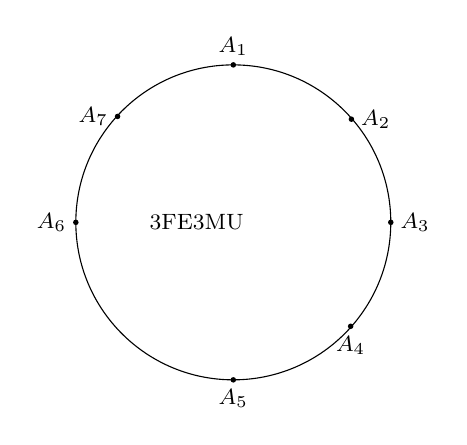
\begin{tikzpicture}[font=\footnotesize, line join=round, line cap=round, >=stealth,scale=0.5]
    %hidden: VM005
				\coordinate (A) at (0,4);
				\coordinate (B) at (3,2.62);
				\coordinate (C) at (4,0);
				\coordinate (D) at (2.98,-2.64);
				\coordinate (E) at (0,-4);
				\coordinate (F) at (-4,0);
				\coordinate (G) at (-2.94,2.69);
				\draw (0,0) circle (4cm);
				\fill (0,4) circle (2pt) node[above]{$A_1$};
				\fill (3,2.62) circle (2pt) node[right]{$A_2$};
				\fill (4,0) circle (2pt) node[right]{$A_3$};
				\fill (2.98,-2.64) circle (2pt) node[below]{$A_4$};
				\fill (0,-4) circle (2pt) node[below]{$A_5$};
				\fill (-4,0) circle (2pt) node[left]{$A_6$};
				\fill (-2.94,2.69) circle (2pt) node[left]{$A_7$};
    \node at (0,0){\href{3FE3MU}{\tiny \phantom{3FE3MU}}};
			\end{tikzpicture}
		\end{center}
		Giả sử ba mã đề khác nhau là $A$, $B$, $C$. \\
		Do vai trò của các mã đề như nhau nên ta xét với mã đề $A$. \\
		Gọi $a$ là số mã đề $A$ được phát. \\
		Nếu $a=0$ thì ta phát các đề $B$, $C$ cho bảy học sinh. Do số học sinh là lẻ nên chắc chắn có hai bạn ngồi gần nhau được phát trùng đề (kiểu $BB$ hoặc $CC$). Do vậy trường hợp này không thỏa mãn. \\ 
		Tương tự với $a=4$ cũng không thỏa mãn. \\
		Khi đó $1 \leq a \leq 3$. 
		\begin{itemize}
			\item Với $a=1$, ta có $7$ cách phát mã $A$. Giả sử phát mã đề $A$ vào vị trí $A_1$, khi đó ta có hai cách phát mã đề $B$, $C$ như sau 
			\begin{center}
				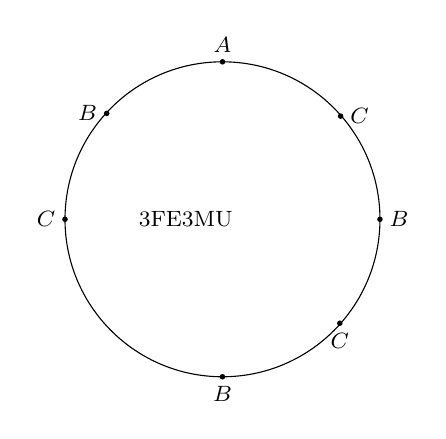
\begin{tikzpicture}[font=\footnotesize, line join=round, line cap=round, >=stealth,scale=0.5]
    %hidden: VM005
					\coordinate (A) at (0,4);
					\coordinate (B) at (3,2.62);
					\coordinate (C) at (4,0);
					\coordinate (D) at (2.98,-2.64);
					\coordinate (E) at (0,-4);
					\coordinate (F) at (-4,0);
					\coordinate (G) at (-2.94,2.69);
					\draw (0,0) circle (4cm);
					\fill (0,4) circle (2pt) node[above]{$A$};
					\fill (3,2.62) circle (2pt) node[right]{$C$};
					\fill (4,0) circle (2pt) node[right]{$B$};
					\fill (2.98,-2.64) circle (2pt) node[below]{$C$};
					\fill (0,-4) circle (2pt) node[below]{$B$};
					\fill (-4,0) circle (2pt) node[left]{$C$};
					\fill (-2.94,2.69) circle (2pt) node[left]{$B$};
    \node at (0,0){\href{3FE3MU}{\tiny \phantom{3FE3MU}}};
				\end{tikzpicture}
				\hspace{2cm}
				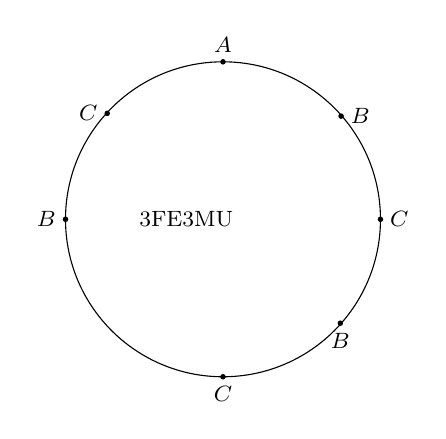
\begin{tikzpicture}[font=\footnotesize, line join=round, line cap=round, >=stealth,scale=0.5]
    %hidden: VM005
					\coordinate (A) at (0,4);
					\coordinate (B) at (3,2.62);
					\coordinate (C) at (4,0);
					\coordinate (D) at (2.98,-2.64);
					\coordinate (E) at (0,-4);
					\coordinate (F) at (-4,0);
					\coordinate (G) at (-2.94,2.69);
					\draw (0,0) circle (4cm);
					\fill (0,4) circle (2pt) node[above]{$A$};
					\fill (3,2.62) circle (2pt) node[right]{$B$};
					\fill (4,0) circle (2pt) node[right]{$C$};
					\fill (2.98,-2.64) circle (2pt) node[below]{$B$};
					\fill (0,-4) circle (2pt) node[below]{$C$};
					\fill (-4,0) circle (2pt) node[left]{$B$};
					\fill (-2.94,2.69) circle (2pt) node[left]{$C$};
    \node at (0,0){\href{3FE3MU}{\tiny \phantom{3FE3MU}}};
				\end{tikzpicture}
			\end{center}
			Do ta có $7$ cách phát mã đề $A$ và với mỗi cách phát đề $A$ có hai cách phát các mã $B$, $C$ nên số cách phát đề trong trường hợp này là $14$ cách. 
			\item Với $a=2$, ta có $\mathrm{C}^{2}_{7}$ cách phát mã $A$, nhưng có $7$ trường hợp hai mã $A$ nằm cạnh nhau nên số cách phát mã $A$ thỏa mãn yêu cầu là $\mathrm{C}^{2}_{7} - 7 = 14$ cách. \\
			Giả sử ta phát mã $A$ vào vị trí $A_1$ và $A_3$, khi đó ta có các cách phát mã $B$, $C$ như sau 
			\begin{center}
				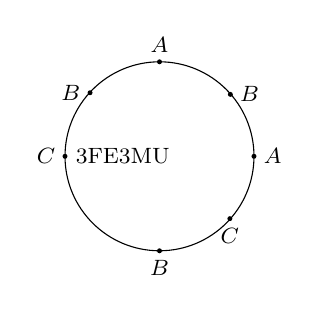
\begin{tikzpicture}[font=\footnotesize, line join=round, line cap=round, >=stealth,scale=0.3]
    %hidden: VM005
					\coordinate (A) at (0,4);
					\coordinate (B) at (3,2.62);
					\coordinate (C) at (4,0);
					\coordinate (D) at (2.98,-2.64);
					\coordinate (E) at (0,-4);
					\coordinate (F) at (-4,0);
					\coordinate (G) at (-2.94,2.69);
					\draw (0,0) circle (4cm);
					\fill (0,4) circle (3pt) node[above]{$A$};
					\fill (3,2.62) circle (3pt) node[right]{$B$};
					\fill (4,0) circle (3pt) node[right]{$A$};
					\fill (2.98,-2.64) circle (3pt) node[below]{$C$};
					\fill (0,-4) circle (3pt) node[below]{$B$};
					\fill (-4,0) circle (3pt) node[left]{$C$};
					\fill (-2.94,2.69) circle (3pt) node[left]{$B$};
    \node at (0,0){\href{3FE3MU}{\tiny \phantom{3FE3MU}}};
				\end{tikzpicture}
				\hfill
				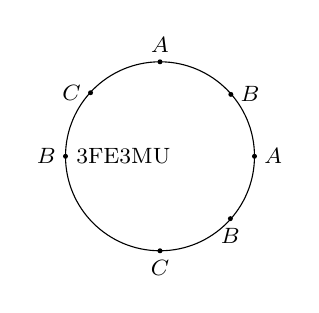
\begin{tikzpicture}[font=\footnotesize, line join=round, line cap=round, >=stealth,scale=0.3]
    %hidden: VM005
					\coordinate (A) at (0,4);
					\coordinate (B) at (3,2.62);
					\coordinate (C) at (4,0);
					\coordinate (D) at (2.98,-2.64);
					\coordinate (E) at (0,-4);
					\coordinate (F) at (-4,0);
					\coordinate (G) at (-2.94,2.69);
					\draw (0,0) circle (4cm);
					\fill (0,4) circle (3pt) node[above]{$A$};
					\fill (3,2.62) circle (3pt) node[right]{$B$};
					\fill (4,0) circle (3pt) node[right]{$A$};
					\fill (2.98,-2.64) circle (3pt) node[below]{$B$};
					\fill (0,-4) circle (3pt) node[below]{$C$};
					\fill (-4,0) circle (3pt) node[left]{$B$};
					\fill (-2.94,2.69) circle (3pt) node[left]{$C$};
    \node at (0,0){\href{3FE3MU}{\tiny \phantom{3FE3MU}}};
				\end{tikzpicture}
				\hfill 
				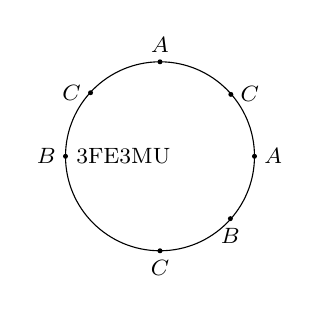
\begin{tikzpicture}[font=\footnotesize, line join=round, line cap=round, >=stealth,scale=0.3]
    %hidden: VM005
					\coordinate (A) at (0,4);
					\coordinate (B) at (3,2.62);
					\coordinate (C) at (4,0);
					\coordinate (D) at (2.98,-2.64);
					\coordinate (E) at (0,-4);
					\coordinate (F) at (-4,0);
					\coordinate (G) at (-2.94,2.69);
					\draw (0,0) circle (4cm);
					\fill (0,4) circle (3pt) node[above]{$A$};
					\fill (3,2.62) circle (3pt) node[right]{$C$};
					\fill (4,0) circle (3pt) node[right]{$A$};
					\fill (2.98,-2.64) circle (3pt) node[below]{$B$};
					\fill (0,-4) circle (3pt) node[below]{$C$};
					\fill (-4,0) circle (3pt) node[left]{$B$};
					\fill (-2.94,2.69) circle (3pt) node[left]{$C$};
    \node at (0,0){\href{3FE3MU}{\tiny \phantom{3FE3MU}}};
				\end{tikzpicture}
				\hfill
				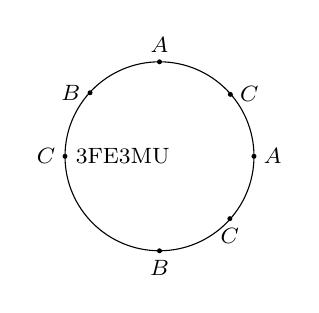
\begin{tikzpicture}[font=\footnotesize, line join=round, line cap=round, >=stealth,scale=0.3]
    %hidden: VM005
					\coordinate (A) at (0,4);
					\coordinate (B) at (3,2.62);
					\coordinate (C) at (4,0);
					\coordinate (D) at (2.98,-2.64);
					\coordinate (E) at (0,-4);
					\coordinate (F) at (-4,0);
					\coordinate (G) at (-2.94,2.69);
					\draw (0,0) circle (4cm);
					\fill (0,4) circle (3pt) node[above]{$A$};
					\fill (3,2.62) circle (3pt) node[right]{$C$};
					\fill (4,0) circle (3pt) node[right]{$A$};
					\fill (2.98,-2.64) circle (3pt) node[below]{$C$};
					\fill (0,-4) circle (3pt) node[below]{$B$};
					\fill (-4,0) circle (3pt) node[left]{$C$};
					\fill (-2.94,2.69) circle (3pt) node[left]{$B$};
    \node at (0,0){\href{3FE3MU}{\tiny \phantom{3FE3MU}}};
				\end{tikzpicture}
			\end{center}
			Với mỗi cách phát mã $A$, ta có $4$ cách phát mã $B$, $C$. \\
			Vậy số cách trong trường hợp này là $56$ (cách). 
			\item Với $a=3$, ta có $\mathrm{C}^{3}_{7}$ cách phát mã $A$. Tuy nhiên trong đó có $7$ trường hợp ba mã $A$ được phát cạnh nhau. 
			\begin{center}
				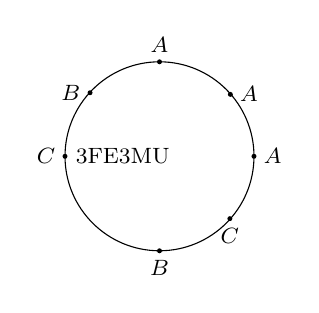
\begin{tikzpicture}[font=\footnotesize, line join=round, line cap=round, >=stealth,scale=0.3]
    %hidden: VM005
					\coordinate (A) at (0,4);
					\coordinate (B) at (3,2.62);
					\coordinate (C) at (4,0);
					\coordinate (D) at (2.98,-2.64);
					\coordinate (E) at (0,-4);
					\coordinate (F) at (-4,0);
					\coordinate (G) at (-2.94,2.69);
					\draw (0,0) circle (4cm);
					\fill (0,4) circle (3pt) node[above]{$A$};
					\fill (3,2.62) circle (3pt) node[right]{$A$};
					\fill (4,0) circle (3pt) node[right]{$A$};
					\fill (2.98,-2.64) circle (3pt) node[below]{$C$};
					\fill (0,-4) circle (3pt) node[below]{$B$};
					\fill (-4,0) circle (3pt) node[left]{$C$};
					\fill (-2.94,2.69) circle (3pt) node[left]{$B$};
    \node at (0,0){\href{3FE3MU}{\tiny \phantom{3FE3MU}}};
				\end{tikzpicture}
				\hfill
				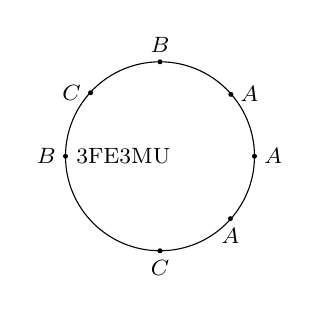
\begin{tikzpicture}[font=\footnotesize, line join=round, line cap=round, >=stealth,scale=0.3]
    %hidden: VM005
					\coordinate (A) at (0,4);
					\coordinate (B) at (3,2.62);
					\coordinate (C) at (4,0);
					\coordinate (D) at (2.98,-2.64);
					\coordinate (E) at (0,-4);
					\coordinate (F) at (-4,0);
					\coordinate (G) at (-2.94,2.69);
					\draw (0,0) circle (4cm);
					\fill (0,4) circle (3pt) node[above]{$B$};
					\fill (3,2.62) circle (3pt) node[right]{$A$};
					\fill (4,0) circle (3pt) node[right]{$A$};
					\fill (2.98,-2.64) circle (3pt) node[below]{$A$};
					\fill (0,-4) circle (3pt) node[below]{$C$};
					\fill (-4,0) circle (3pt) node[left]{$B$};
					\fill (-2.94,2.69) circle (3pt) node[left]{$C$};
    \node at (0,0){\href{3FE3MU}{\tiny \phantom{3FE3MU}}};
				\end{tikzpicture}
				\hfill 
				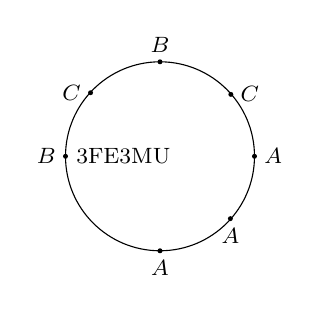
\begin{tikzpicture}[font=\footnotesize, line join=round, line cap=round, >=stealth,scale=0.3]
    %hidden: VM005
					\coordinate (A) at (0,4);
					\coordinate (B) at (3,2.62);
					\coordinate (C) at (4,0);
					\coordinate (D) at (2.98,-2.64);
					\coordinate (E) at (0,-4);
					\coordinate (F) at (-4,0);
					\coordinate (G) at (-2.94,2.69);
					\draw (0,0) circle (4cm);
					\fill (0,4) circle (3pt) node[above]{$B$};
					\fill (3,2.62) circle (3pt) node[right]{$C$};
					\fill (4,0) circle (3pt) node[right]{$A$};
					\fill (2.98,-2.64) circle (3pt) node[below]{$A$};
					\fill (0,-4) circle (3pt) node[below]{$A$};
					\fill (-4,0) circle (3pt) node[left]{$B$};
					\fill (-2.94,2.69) circle (3pt) node[left]{$C$};
    \node at (0,0){\href{3FE3MU}{\tiny \phantom{3FE3MU}}};
				\end{tikzpicture}
				\ldots \ldots \hfill
				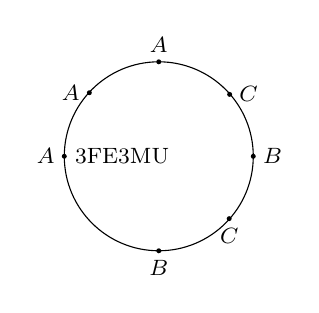
\begin{tikzpicture}[font=\footnotesize, line join=round, line cap=round, >=stealth,scale=0.3]
    %hidden: VM005
					\coordinate (A) at (0,4);
					\coordinate (B) at (3,2.62);
					\coordinate (C) at (4,0);
					\coordinate (D) at (2.98,-2.64);
					\coordinate (E) at (0,-4);
					\coordinate (F) at (-4,0);
					\coordinate (G) at (-2.94,2.69);
					\draw (0,0) circle (4cm);
					\fill (0,4) circle (3pt) node[above]{$A$};
					\fill (3,2.62) circle (3pt) node[right]{$C$};
					\fill (4,0) circle (3pt) node[right]{$B$};
					\fill (2.98,-2.64) circle (3pt) node[below]{$C$};
					\fill (0,-4) circle (3pt) node[below]{$B$};
					\fill (-4,0) circle (3pt) node[left]{$A$};
					\fill (-2.94,2.69) circle (3pt) node[left]{$A$};
    \node at (0,0){\href{3FE3MU}{\tiny \phantom{3FE3MU}}};
				\end{tikzpicture}
			\end{center}
			và $7 \cdot 3 =21$ cách phát có $2$ mã $A$ cạnh nhau (dạng tam giác). \\
			Do vậy số cách phát mã $A$ thỏa mãn yêu cầu là $\mathrm{C}^{3}_{7} - 7 \cdot 3 - 7 =7$ cách. \\
			Với mỗi cách phát mã $A$, ta có $2^3$ cách phát mã $B$, $C$. \\
			Vậy số cách trong trường hợp này là $56$ (cách). 
		\end{itemize}
		Vậy số cách phát đề là $14 + 56 + 56 = 126$ (cách). 
	}
\end{ex}

\begin{ex}%[Dự án 29OH5N-VN-MT-15]%[2-KS-18-SoQuangNinh-L1-2026, TV035]%[2H5V2-8]
	Trong không gian $Oxyz$, cho hai điểm $A(6; 0; 4)$, $B(-3; -2; 1)$ và mặt phẳng $(P)$ có phương trình $x + y + 5z +1 =0$. Biết điểm $M$ là điểm thuộc mặt phẳng $(P)$ sao cho $MA + MB$ đạt giá trị nhỏ nhất, tính độ dài đoạn $OM$ (\textit{không làm tròn các bước trung gian, chỉ làm tròn kết quả cuối cùng đến hàng phần trăm}). 
	\par \shortans{$3{,}48$}
	\loigiai{
		Vì $6 + 0 + 5 \cdot 4 + 1 = 27>0$ và $-3 + (-2) + 5 \cdot 1 + 1 =1 >0$ nên $A$ và $B$ nằm về cùng một phía đối với mặt phẳng $(P)$. \\
		Gọi $H$ là hình chiếu của điểm $A$ xuống mặt phẳng $(P)$.\\
		Đường thẳng $AH$ đi qua điểm $A$ và vuông góc mặt phẳng $(P)$ nên có phương trình là $\heva{& x = 6 + t \\ & y = t \\ & z = 4 + 5t}$ với $t \in \mathbb{R}$. \\ 
		Do đó, tọa độ $H$ có dạng $H(6+t; t; 4+5t)$. \\
		Vì $H \in (P)$ nên $6+t + t + 5 \cdot (4 +5t) + 1 =0 \Leftrightarrow t =-1 \Rightarrow H (5; -1; -1)$. \\
		Gọi $A'$ là điểm đối xứng của điểm $A$ qua mặt phẳng $(P)$. Ta được $A' (4; -2; -6)$. \\
		Ta có $MA + MB = MA' + MB \geq A'B$. \\
		Suy ra $MA + MB$ nhỏ nhất khi và chỉ khi $M$ là giao điểm của $A'B$ với $(P)$. \\
		Ta có $\overrightarrow{A'B} = (-7; 0; 7)$. Suy ra $\overrightarrow{u} = (1; 0; -1)$ là một vectơ chỉ phương của đường thẳng $A'B$. \\
		Suy ra phương trình đường thẳng $A'B$ là $\heva{& x = 4 + t \\ & y=-2 \\& z = -6 - t}$ với $t \in \mathbb{R}$. \\
		Tọa độ điểm $M$ là nghiệm của hệ $\heva{& x = 4 + t \\ & y=-2 \\& z = -6 - t \\ & x + y + 5z + 1 =0} \Leftrightarrow \heva{& t = - \dfrac{27}{4} \\ & x = - \dfrac{11}{4} \\ & y =-2 \\ & z = \dfrac{3}{4}.}$ \\
		Vậy $M \left(-\dfrac{11}{4}; -2; \dfrac{3}{4}\right) \Rightarrow OM = \sqrt{\left(- \dfrac{11}{4} \right)^2 + (-2)^2 + \left(\dfrac{3}{4} \right)^2} = \dfrac{\sqrt{194}}{4} \approx 3{,}48$. 
	}
\end{ex}

\begin{ex}%[Dự án 2LHA5B-VN-MT-15]%[2-KS-18-SoQuangNinh-L1-2026, TV035]%[2D4H2-6]
	Vệ tinh Van Allen Probes được phóng lên không gian để nghiên cứu các vành đai bức xạ bao quanh Trái Đất. Vệ tinh này bay theo một quỹ đạo có chu kỳ $10$ giờ - nghĩa là mỗi vòng bay quanh trái đất kéo dài đúng $10$ giờ. Cứ mỗi vòng bay, vệ tinh lại xuyên qua vùng bức xạ mạnh và tích lũy thêm {\it liều bức xạ}. Biết rằng đơn vị của bức xạ là Gray (Gy), và khi tổng {\it liều bức xạ} chiếu vào vệ tinh đạt $1\,000$ Gray, thì vệ tinh hỏng hoàn toàn. Khoảng cách từ tâm trái đất đến vệ tinh được mô hình hóa bằng hàm số $R (T) = 7\,000 + 3\,000T$\,(km), trong đó $T$ là thời gian tính bằng giờ, $0 \leq T \leq 10$, kể từ đầu vòng bay. Công thức {\it suất liều bức xạ} - tức là lượng bức xạ vệ tinh nhận trong $1$ giờ, phụ thuộc vào khoảng cách $R$\,(km) từ vệ tinh đến Trái Đất, là $D (R) = 60 \cdot \left(\dfrac{R}{25\,000}\right)^2$ milligray/giờ. Biết rằng do tính đối xứng và chu kỳ của quỹ đạo bay, tổng liều bức xạ vệ tinh nhận được trong một vòng bay $10$ giờ được tính bằng công thức $L = 2 \cdot \displaystyle \int\limits_{0}^{5} D (R(T)) \mathrm{d}T$, và $1$ Gray $=1\,000$ milligray. Tính số năm hoạt động của vệ tinh từ lúc bắt đầu hoạt động tới khi hỏng hoàn toàn \textit{(không làm tròn các bước trung gian, chỉ làm tròn kết quả cuối cùng đến hai chữ số thập phân sau dấu phẩy, coi một năm có $365$ ngày, mỗi ngày có $24$ giờ}). 
	\par \shortans{$5{,}19$}
	\loigiai{
		Tổng liều bức xạ vệ tinh nhận được trong một vòng bay $10$ giờ là 
		\[
		L = 2 \cdot \displaystyle \int\limits_{0}^{5} 60 \cdot \left(\dfrac{7\,000 + 3\,000T}{25\,000}\right)^2 \mathrm{d}T=219{,}84 \text{ (milligray)}. 
		\]
		Vậy sau $1$ giờ, vệ tinh nhận được $21{,}984$ milligray bức xạ. \\
		Vậy tuổi thọ của vệ tinh là $\dfrac{10^6}{21{,}984 \cdot 365 \cdot 24} \approx 5{,}19$ (năm). 
	}
\end{ex}

\begin{ex}%[Dự án 4LSAFW-VN-MT-15]%[2-KS-18-SoQuangNinh-L1-2026, VM006]%[1D6V4-6]
	Trong âm nhạc, một \textit{quãng tám} (octave) là khoảng cách âm thanh từ nốt Đô tới nốt Đô tiếp theo, theo thứ tự từ thấp đến cao là
	\begin{center}
		Đô - Đô\,\# - Rê  - Rê\,\# - Mi (E$4$) - Pha - Pha\,\# - Sol - Sol\,\# - La (A$4$) - La\,\# - Si - Đô
	\end{center}
	trong đó khoảng cách giữa hai nốt liên tiếp gọi là một nửa cung (semitone). Hai nốt cách nhau $n$ nửa cung thì tỉ lệ tần số nốt cao $f_{\text{nc}}$ và tần số nốt thấp $f_{\text{nt}}$ là $\dfrac{f_{\text{nc}}}{f_{\text{nt}}}=2^{\tfrac{n}{12}}$; cho biết tần số của nốt La (A$4$) là $440$\,Hz. Trên đàn guitar, dây số $1$ là nốt Mi (E$4$) đang bị chùng do thời tiết, tần số đo được hiện tại đang là $300$\,Hz. Để căng lại dây đàn cho chuẩn, ta dùng núm xoay và cứ vặn núm xoay $90^\circ$ thì nốt nhạc được tăng lên một nửa cung. Hỏi phải xoay núm dây số $1$ một góc bao nhiêu độ để dây số $1$ trở về âm chuẩn (\textit{không làm tròn các bước trung gian, chỉ làm tròn kết quả cuối cùng tới hàng đơn vị})?
	\par \shortans{$147$}
	\loigiai{
		Nốt La (A$4$) cách nốt Mi (E$4$) đúng $5$ nửa cung nên tần số của nốt Mi (E$4$) bằng $\dfrac{440}{2^{\tfrac{5}{12}}}$ (Hz).\\
		Để căng lại dây đàn số $1$ cho chuẩn, ta cần xoay núm xoay $n$ nửa cung thỏa mãn
		\[\dfrac{\dfrac{440}{2^{\tfrac{5}{12}}}}{300}=2^{\tfrac{n}{12}}\Leftrightarrow n=12\log_2\left(\dfrac{22}{15\cdot 2^{\tfrac{5}{12}}}\right).\]
		Do đó phải xoay núm dây số $1$ một góc 
		\[
		90\cdot12\log_2\left(\dfrac{22}{15\cdot 2^{\tfrac{5}{12}}}\right)\approx147^\circ.
		\]
	}
\end{ex}

\begin{ex}%[Dự án 41WIB7-VN-MT-15]%[2-KS-18-SoQuangNinh-L1-2026, VM006]%[2D1V3-6]
	Mô hình \textit{EOQ} (Economic Order Quantity) được công bố năm $1913$ là một công cụ quản trị vận hành dùng để xác định lượng hàng nhập kho tối ưu. Giả sử một cửa hàng thức ăn cho mèo có nhu cầu tiêu thụ hàng hóa đều đặn với tốc độ bán hàng $d=100$ hộp/ngày. các thông số chi phí được xác định như sau:
	\begin{itemize} 
		\item $K=1\,000\,000$ đồng là chi phí cố định cho mỗi lần đặt hàng (phí vận chuyển, nhân công,...);
		\item $c$ đồng/hộp là giá nhập mỗi hộp hàng (giả định không đổi và không có chiết khấu);
		\item $h=500$ đồng/hộp/ngày là đơn giá lưu kho (chi phí lưu giữ một hộp hàng trong kho trong một ngày).
	\end{itemize}
	Gọi $Q$ (hộp) là số lượng hàng mà người bán nhập vào trong kho mỗi lần đặt hàng. Thời gian tiêu thụ hết lượng hàng là $\dfrac{Q}{d}$ (ngày). Tổng chi phí cho một chu kì đặt hàng và tiêu thụ hết hàng là $f=K+cQ+\dfrac{hQ^2}{2d}$. Hỏi cửa hàng nên nhập bao nhiêu hộp trong mỗi lần đặt hàng để chi phí trung bình mỗi ngày là nhỏ nhất (\textit{không làm tròn các bước trung gian, chỉ làm tròn kết quả cuối cùng tới hàng đơn vị})?
	\par \shortans{$632$}
	\loigiai{
		Chi phí trung bình mỗi ngày là 
		\[
		T=\dfrac{f}{\dfrac{Q}{d}}=\dfrac{K+cQ+\dfrac{hQ^2}{2d}}{\dfrac{Q}{d}}=\dfrac{Kd}{Q}+cd+\dfrac{hQ}{2}.
		\]
		Xét hàm số $T(Q)=\dfrac{Kd}{Q}+cd+\dfrac{hQ}{2}$, với $Q>0$.\\
		Vì $K$, $d$, $c$, $h$ là hằng số nên ta có $T'(Q)=\dfrac{-Kd}{Q^2}+\dfrac{h}{2}$.\\
		Xét $T'(Q)=0\Rightarrow Q=\sqrt{\dfrac{2Kd}{h}}=200\sqrt{10}$.\\
		Bảng biến thiên 
		\begin{center}
			\begin{tikzpicture}
    %hidden: VM005
				\tkzTabInit[nocadre=true, lgt=1.3, espcl=4, deltacl=0.5]
				{$Q$/0.7,$T’(Q)$/0.7,$T(Q)$/2}
				{$0$,$200\sqrt{10}$,$+\infty$}
				\tkzTabLine{,-,0,+,}
				\tkzTabVar{+/$+\infty$,-/$T\left(200\sqrt{10}\right)$,+/$+\infty$}
    \node at (T11){\href{41WIB7}{\tiny \phantom{41WIB7}}};
			\end{tikzpicture}
		\end{center}
		Dựa vào bảng biến thiên, $T$ đạt giá trị nhỏ nhất khi $Q=200\sqrt{10}\approx 632$.\\
		Vậy cửa hàng nên nhập khoảng $632$ hộp trong mỗi lần đặt hàng để chi phí trung bình mỗi ngày là nhỏ nhất.
	}
\end{ex}

\begin{ex}%[Dự án 5XUO5I-VN-MT-15]%[2-KS-18-SoQuangNinh-L1-2026, VM006]%[1H8V5-3]
	Cho hình lăng trụ $ABC.A'B'C'$ có đáy $ABC$ là tam giác đều cạnh bằng $2$, hình chiếu của $A'$ trên $(ABC)$ trùng với trung điểm $M$ của $AB$; góc giữa cạnh bên và mặt đáy bằng $60^\circ$. Gọi $N$ là trung điểm của $CC'$. Tính khoảng cách từ $B'$ tới mặt phẳng $\left(A'MN\right)$ (\textit{không làm tròn các bước trung gian, chỉ làm tròn kết quả cuối cùng tới hàng phần trăm})?
	\par \shortans{$1{,}92$}
	\loigiai{
		\begin{center}
			\begin{tikzpicture}[font=\footnotesize, line join=round, line cap=round, >=stealth, scale=1] 
    %hidden: VM005
				\def\a{3}
				\def\h{3}
				\path 	(0:0) coordinate (A)
					++(0:\a) coordinate (C)
					++(-150:3*\a/4) coordinate (B)
					($(A)!0.5!(B)$) coordinate (M)
					($(M)+(90:\h)$) coordinate (A')
					($(B)+1*(A')-1*(A)$) coordinate (B')
					($(C)+1*(A')-1*(A)$) coordinate (C')
					($(C)!0.5!(C')$) coordinate (N)
					(intersection of A'--N and A--C) coordinate (P)
					(intersection of M--P and B--C) coordinate (I)
					(intersection of A--B' and A'--M) coordinate (E)
					;
				\draw[dashed] 	(A)--(P) (M)--(N)--(A') (M)--(P) (I)--(C)--(N);
				\draw	(N)--(C') 	(B)--(B')	(A)--(A') (A)--(B)--(I) (A')--(B')--(C')--cycle (A')--(M) (N)--(P) (I)--(P) (A)--(B');
				\foreach \x/\g in {A/180,B/-45,C/45,A'/180,B'/-45,C'/0,M/-120,N/30,P/0,E/-45}\fill (\x) circle (1pt) ($(\g:3mm)+(\x)$) node {$\x$};	
    \node at (0,0){\href{5XUO5I}{\tiny \phantom{5XUO5I}}};
			\end{tikzpicture}
		\end{center}
		Ta có $AM$ là hình chiếu vuông góc của $AA'$ lên mặt phẳng $(ABC)$.\\
		Suy ra $\big(AA',(ABC)\big)=\left(AA',AM\right)=\widehat{A'AM}=60^\circ\Rightarrow A'M=AM\cdot \tan 60^\circ=\sqrt{3}$.\\
		Trong mặt phẳng $\left(ACC'A'\right)$ gọi $P$ là giao điểm của $A'N$ và $AC$, suy ra $AP=2AC=4$.\\
		Trong mặt phẳng $\left(ABB'A'\right)$ gọi $E$ là giao điểm của $A'M$ và $AB'$, suy ra $\dfrac{B'E}{AE}=\dfrac{A'B'}{AM}=2$.\\
		Ta có $\mathrm{d}\left(B',\left(A'MP\right)\right)=\dfrac{B'E}{AE}\cdot\mathrm{d}\left(A,\left(A'MP\right)\right)=2\mathrm{d}\left(A,\left(A'MP\right)\right)$.\\
		Mặt phẳng $\left(A'MP\right)$ chứa $A'M$ vuông góc với mặt phẳng $(ABC)$ nên $\left(A'MP\right)\perp (ABC)$.\\
		Suy ra 
		\allowdisplaybreaks
		\begin{align*} 
			\mathrm{d}\left(A,\left(A'MP\right)\right)&=\mathrm{d}(A,MP)  \\ 
			&=\dfrac{2S_{\triangle AMP}}{MP}  \\ 
			&=\dfrac{AM\cdot AP\cdot \sin\widehat{MAP}}{\sqrt{AM^2+AP^2-2AM\cdot AP\cdot\cos\widehat{MAP}}}  \\ 
			&=\dfrac{1 \cdot 4\cdot \sin 60^\circ}{\sqrt{1^2+4^2-2\cdot 1\cdot 4\cdot\cos 60^\circ}}  \\ 
			&=\dfrac{2\sqrt{39}}{13}.
		\end{align*}
		Do đó, $\mathrm{d}\left(B',\left(A'MN\right)\right)=\mathrm{d}\left(B',\left(A'MP\right)\right)=\dfrac{4\sqrt{39}}{13}\approx 1{,}92$.
	}
\end{ex}

\Closesolutionfile{ans}
\Closesolutionfile{ansbook}
\begin{indapan}
	{ans/ans\currfilebase}
\end{indapan}